\documentclass[tikz,border=9pt]{standalone}
\usepackage[T1]{fontenc}\usepackage{lmodern,amsmath,amssymb}
\usetikzlibrary{arrows.meta,positioning,calc}
\begin{document}
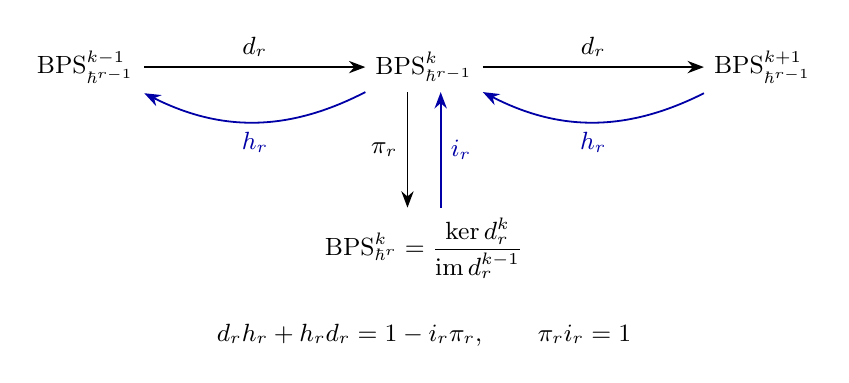
\begin{tikzpicture}[>=Stealth, every node/.style={font=\small},every path/.style={line width=.65pt}]

\node (a) at (-4.3,1.1) {$\mathrm{BPS}_{\hbar^{r-1}}^{k-1}$};
\node (b) at (0,1.1) {$\mathrm{BPS}_{\hbar^{r-1}}^{k}$};
\node (c) at (4.3,1.1) {$\mathrm{BPS}_{\hbar^{r-1}}^{k+1}$};
\draw[->] (a.east) -- node[above] {$d_r$} (b.west);
\draw[->] (b.east) -- node[above] {$d_r$} (c.west);
\draw[->,blue!65!black] (b.south west) to[bend left=27] node[below] {$h_r$} (a.south east);
\draw[->,blue!65!black] (c.south west) to[bend left=27] node[below] {$h_r$} (b.south east);
\node (d) at (0,-1.2) {$\displaystyle\mathrm{BPS}_{\hbar^r}^{k}=\frac{\ker d_r^{k}}{\operatorname{im}d_r^{k-1}}$};
\draw[->] ([xshift=-6pt]b.south) -- node[left] {$\pi_r$} ([xshift=-6pt]d.north);
\draw[->,blue!65!black] ([xshift=6pt]d.north) -- node[right] {$i_r$} ([xshift=6pt]b.south);
\node at (0,-2.3) {$d_rh_r+h_rd_r=1-i_r\pi_r,\qquad \pi_ri_r=1$};

\end{tikzpicture}
\end{document}
